% ============================================================================
% presentation.tex
% Beamer deck for: Liquidity, Activism Disclosure, and Takeover Premia
% 14 core slides + 27 backup slides with bidirectional hyperlinks
% ============================================================================
%
% ── AUDIENCE CALIBRATION NOTE ──────────────────────────────────────────────
%
% Professor Alex Gorbenko (Primary supervisor, UCL)
%   Published: JF (2014, 2024), AER (2011), RFS (2010, 2013, 2018),
%     JFE (2019, 2022). Key papers on M&A auctions, strategic vs financial
%     bidders, deal initiation, CDS auctions, VC contracts.
%   Research profile: Theory + structural estimation in corporate control.
%     Co-Director of MSc Law & Finance. Values law & finance intersections,
%     institutional design, and policy-relevant implications.
%   Calibration: Frame disclosure policy and testable predictions as
%     first-class results. Connect equilibrium mechanics to Schedule 13D,
%     FCA thresholds, SEC filing window debates. His 2024 JF paper on
%     endogenous auction initiation parallels our disclosure threshold
%     (information revelation through action choice).
%
% Professor Ming Yang (Second supervisor, UCL)
%   Published: REStud (2020, 2022), RFS (2019, 2024), TE (2020),
%     JET (2015), JAE (2017), MS (2024). Key papers on rational inattention,
%     security design under flexible info acquisition, coordination games.
%   Research profile: Microeconomic theorist at the boundary of information
%     economics and finance. Distinctive contribution: applying rational
%     inattention to corporate finance. Works with Stephen Morris (REStud 2022)
%     on coordination and global games.
%   Calibration: State propositions formally. Do not hand-wave the contraction
%     mapping or fixed-point arguments. The Bayesian inference mechanics
%     (Proposition 2) are where the model's information-theoretic content
%     lives. The noisy rumor extension echoes his interest in information
%     structures. He will probe single-crossing logic and whether comparative
%     statics are grounded in primitives.
%
% Design principle: Every slide must simultaneously satisfy a theorist who
% will stress-test equilibrium foundations (Yang) and a corporate-finance
% economist who will ask "what does this mean for SEC policy?" (Gorbenko).
% ============================================================================

\documentclass[aspectratio=169,11pt]{beamer}

\usetheme{ucl}
\useoutertheme[small]{ucltitlebanner}

% Title page style
\setbeamercolor{title}{fg=black,bg=}
\setbeamerfont{frametitle}{series=\bfseries}

% Packages
\usepackage{amsmath,amssymb,amsfonts}
\usepackage{booktabs}
\usepackage{graphicx}
\usepackage{array}
\usepackage{tabularx}
\usepackage{multirow}
\usepackage{tikz}
\usetikzlibrary{arrows.meta,positioning,shapes.geometric,calc,decorations.pathreplacing}
\usepackage{csquotes}
\usepackage{hyperref}

\usepackage[backend=biber,style=authoryear,natbib=true,maxcitenames=2,maxbibnames=99]{biblatex}
\addbibresource{slides.bib}

% Notation macros
\newcommand{\E}{\mathbb{E}}
\newcommand{\PP}{\mathbb{P}}
\newcommand{\1}{\mathbf{1}}
\newcommand{\Var}{\mathrm{Var}}
\newcommand{\R}{\mathbb{R}}

% Color coding for notation categories
\usepackage{xcolor}
\newcommand{\choice}[1]{\textcolor{blue}{#1}}
\newcommand{\obs}[1]{\textcolor{red!70!black}{#1}}
\newcommand{\outcome}[1]{\textcolor{green!50!black}{#1}}

% Hyperlink styling
\hypersetup{colorlinks=true, linkcolor=brightblue, urlcolor=brightblue}

% Backup slide navigation helper
\newcommand{\backuplink}[2]{%
  \hfill{\scriptsize\hyperlink{#1}{\textcolor{brightblue}{#2\,$\nearrow$}}}%
}
\newcommand{\returnlink}[2]{%
  \par\vspace{0.2em}\hfill{\scriptsize\hyperlink{#1}{\textcolor{brightblue}{$\leftarrow$\,#2}}}%
}

% Beamer cosmetics
\setbeamertemplate{navigation symbols}{}
\setbeamertemplate{footline}[author title date]

% Block style
\setbeamercolor{block title}{fg=brightblue,bg=}
\setbeamercolor{block body}{fg=black,bg=}
\setbeamerfont{block title}{series=\bfseries}
\setbeamertemplate{block begin}{%
  \par\vskip\smallskipamount%
  {\usebeamerfont*{block title}\usebeamercolor[fg]{block title}\insertblocktitle\par}%
  \vspace{0.2ex}%
  {\usebeamercolor[fg]{block title}\rule{\linewidth}{0.4pt}\par}%
  \begin{beamercolorbox}[wd=\linewidth,sep=0.6ex]{block body}%
    \usebeamerfont{block body}%
}
\setbeamertemplate{block end}{%
  \end{beamercolorbox}%
  \vskip\smallskipamount%
}

% Graphics path
\graphicspath{{figures/}}

% Title
\title[Liquidity, Activism, Takeover Premia]{\textbf{Liquidity, Activism Disclosure, and Takeover Premia:}\\[0.2em]
\large A Theory of Exit, Voice, and Corporate Control}
\author[Austin Li]{Austin Li}
\institute[]{University College London}
\date[]{}

\begin{document}

% ============================================================================
% TITLE SLIDE
% ============================================================================

\begin{frame}
  \titlepage
\end{frame}

% ============================================================================
% CORE DECK: 13 SLIDES
% ============================================================================

% ── SLIDE 1: Motivating Facts & Central Question ──────────────────────────
\begin{frame}{Activist Returns and the Takeover Channel}
\hypertarget{main:motivation}{}
\begin{itemize}\itemsep0.5em
  \item \textbf{\citealp{BravJiangPartnoyThomas2008}:} Roughly 65\% of activist hedge fund returns come from M\&A events
  \item \textbf{\citealp{GreenwoodSchor2009}:} Activist targets are acquired at significant premia; activists profit primarily through the takeover channel
  \item \textbf{\citealp{CollinDufresneFos2015}:} Informed trading before Schedule 13D filings moves prices; activists trade strategically on private information
\end{itemize}

\vspace{0.5em}

\begin{block}{Central Question}
How does market liquidity shape the takeover premia that minority shareholders receive when a blockholder can exit, hold, or engage?
\end{block}
\end{frame}

% ── SLIDE 2: Literature Gap & Contribution ────────────────────────────────
\begin{frame}{Three Literatures, One Missing Piece}
\hypertarget{main:literature}{}
\small
\begin{columns}[T,onlytextwidth]
\column{0.52\textwidth}

{\usebeamerfont*{block title}\usebeamercolor[fg]{block title}\textbf{Exit / Voice}\par}
\vspace{0.2ex}{\usebeamercolor[fg]{block title}\rule{\linewidth}{0.4pt}\par}\vspace{0.3em}
\citealp{Edmans2009}, \citealp{Maug1998}, \citealp{AdmatiPfleiderer2009}: liquidity enables exit-based governance and stake-building for intervention.

\vspace{0.25em}

{\usebeamerfont*{block title}\usebeamercolor[fg]{block title}\textbf{Microstructure \& Feedback}\par}
\vspace{0.2ex}{\usebeamercolor[fg]{block title}\rule{\linewidth}{0.4pt}\par}\vspace{0.3em}
\citealp{Kyle1985}, \citealp{BackEtAl2018}: informed trading, strategic liquidity, and price discovery.

\vspace{0.25em}

{\usebeamerfont*{block title}\usebeamercolor[fg]{block title}\textbf{Takeover \& Real Effects}\par}
\vspace{0.2ex}{\usebeamercolor[fg]{block title}\rule{\linewidth}{0.4pt}\par}\vspace{0.3em}
\citealp{EdmansGoldsteinJiang2012}: prices guide real decisions, including takeover entry.

\column{0.46\textwidth}
\begin{block}{The Gap}
No model links all three: how does market liquidity, through its effect on information in prices, shape takeover premia for minority shareholders?
\end{block}

\vspace{0.2em}

{\small\textbf{Contribution:}\\[0.2em]
(i) Non-monotone liquidity effect on premia\\
(ii) Disclosure attenuation mechanism\\
(iii) Premium wedge from tender mechanics\\
(iv) Liquidity regulation $\equiv$ governance policy}
\end{columns}
\end{frame}

% ── SLIDE 2b: Positioning vs the structural activism trio ────────────────
\begin{frame}{Positioning: The Structural Activism Trio}
\hypertarget{main:positioning}{}
\small
\begin{itemize}\itemsep0.35em
  \item \textbf{\citealp{JohnsonSwem2021}} (JFE): dynamic \emph{reputation}; accumulation is a reduced-form cost draw; owns the 13D-window $\leftrightarrow$ $\sigma^2 T$ lever (2024 acceleration).
  \item \textbf{\citealp{AlbuquerqueFosSchroth2022}} (JFE): structural 13D-vs-13G choice; engagement cost a \emph{scalar}; estimate activism \emph{lowers} bid premia by $13.7\%$.
  \item \textbf{\citealp{CelentanoLevine2025}} (R\&R RFS): equilibrium activism $+$ takeovers $+$ managerial discipline; no market microstructure.
\end{itemize}

\begin{block}{This paper's lane}
\small Liquidity, order-flow inference, and the disclosure rule are the trio's \textbf{missing state variables}. The premium they estimate as a constant is here an \textbf{equilibrium object of tender mechanics} ($\lambda = 1-q(1-\gamma)\psi$) --- and the AFS negative sign is the low-$\lambda$ region of our model, not a contradiction.
\end{block}
\end{frame}

% ── SLIDE 3: Disclosure Creates Two Information Regimes ───────────────────
\begin{frame}{Disclosure Creates Two Information Regimes}
\hypertarget{main:disclosure}{}
\begin{columns}[T,onlytextwidth]
\column{0.54\textwidth}
\textbf{Institutional facts:}
\begin{itemize}\itemsep0.1em
  \item \textbf{US:} 5\% threshold, 10-day filing window (Schedule 13D)
  \item \textbf{UK:} 3\% threshold, 2-day window (FCA TR-1)
  \item Creates two observability regimes:
\end{itemize}

\vspace{0.3em}

\scriptsize
\begin{tabular}{ll}
\toprule
\textbf{Quiet Voice} ($D{=}0$) & \textbf{Public Voice} ($D{=}1$) \\
\midrule
No disclosure triggered & Filing triggers $D{=}1$ \\
Engagement \emph{inferred} from $X$ & Engagement \emph{observed} \\
Inference depends on $\kappa$ & Independent of $\kappa$ \\
\bottomrule
\end{tabular}
\normalsize

\column{0.44\textwidth}
\begin{block}{Model Translation}
\vspace{0.2em}
$D = \1\{q = +1\}$\\[0.3em]
Buy-and-engage $\Rightarrow$ public disclosure\\
Hold-and-engage $\Rightarrow$ no disclosure
\end{block}

\vspace{0.3em}

{\footnotesize Disclosure partitions equilibrium into \textbf{inference} ($D{=}0$, $\kappa$ matters) vs.\ \textbf{observed} ($D{=}1$, $\kappa$ irrelevant) regimes.}

\backuplink{backup:disclosure_regimes}{Alternative regimes}
\end{columns}
\end{frame}

% ── SLIDE 4: Notation Guide ──────────────────────────────────────────────
\begin{frame}{Notation Guide}
\hypertarget{main:notation}{}
\tiny
\begin{columns}[T,onlytextwidth]
\column{0.31\textwidth}
\begin{tabular}{@{}ll@{}}
\toprule
\multicolumn{2}{l}{\textbf{\choice{Choices / Actions}}} \\
\midrule
$\choice{q} \in \{-1,0,+1\}$ & Trade order \\
$\choice{a} \in \{0,1\}$ & Engage? \\
$\choice{z} \in \{-1,0,+1\}$ & Noise trade \\
\midrule
\multicolumn{2}{l}{\textbf{\obs{Observables}}} \\
\midrule
$\obs{X} = q + z$ & Order flow \\
$\obs{D} = \1\{q=+1\}$ & Disclosure \\
$\obs{s} = v + \varepsilon$ & Private signal \\
$\obs{v} \sim N(\mu,\sigma_v^2)$ & Fundamental \\
\bottomrule
\end{tabular}

\column{0.35\textwidth}
\begin{tabular}{@{}ll@{}}
\toprule
\multicolumn{2}{l}{\textbf{\outcome{Equilibrium Objects}}} \\
\midrule
$\outcome{\pi}(X,D)$ & Posterior $\PP(a{=}1|X,D)$ \\
$\outcome{P}(X,D)$ & Equilibrium price \\
$\outcome{p}(P,D)$ & Bid probability \\
$\outcome{m}(X,D)$ & Expected premium \\
\midrule
\multicolumn{2}{l}{\textbf{Cutoffs (Prop.\ 1)}} \\
\midrule
$k_1$ & Exit / Hold \\
$k_0$ & Hold / Quiet Voice \\
$k_D$ & Quiet / Public Voice \\
\bottomrule
\end{tabular}

\column{0.33\textwidth}
\begin{tabular}{@{}ll@{}}
\toprule
\multicolumn{2}{l}{\textbf{Parameters}} \\
\midrule
$\kappa$ & Liquidity (noise) \\
$\rho$ & Engage success prob. \\
$\Delta,\tilde{\Delta}$ & Value-add ($\tilde{\Delta}=\rho\Delta$) \\
$m_0, m_1$ & Premia (base, success) \\
$\tilde{m}$ & $m_0 + \rho(m_1 - m_0)$ \\
$C_0, \chi$ & Engage cost params \\
$\bar{S}, K, \sigma_\xi$ & Bidder entry \\
$\delta$ & Discount factor \\
\midrule
\multicolumn{2}{l}{\textbf{Region probs}} \\
\midrule
$\omega_E,\omega_H,\omega_Q,\omega_P$ & Action probs \\
\bottomrule
\end{tabular}
\end{columns}

\vspace{0.3em}
\centering
{\footnotesize \choice{Blue}\,=\,choices \quad \obs{Red}\,=\,observables \quad \outcome{Green}\,=\,outcomes}
\end{frame}

% ── SLIDE 5: Model Timeline & Actions ─────────────────────────────────────
\begin{frame}{Model Timeline \& Actions}
\hypertarget{main:timeline}{}
\centering
\begin{tikzpicture}[
  stage/.style={circle, draw=brightblue, thick, fill=brightblue!15,
                minimum size=1.0cm, font=\footnotesize\bfseries},
  arr/.style={-Stealth, thick, brightblue!70!black},
  lbl/.style={font=\scriptsize, text width=2.5cm, align=center},
  node distance=2.5cm
]
  \node[stage] (t0) {$t{=}0$};
  \node[stage, right=of t0] (t1) {$t{=}1$};
  \node[stage, right=of t1] (t15) {$t{=}1.5$};
  \node[stage, right=of t15] (t2) {$t{=}2$};
  \draw[arr] (t0) -- (t1);
  \draw[arr] (t1) -- (t15);
  \draw[arr] (t15) -- (t2);
  \node[above=0.25cm of t0, font=\bfseries\footnotesize] {Nature};
  \node[above=0.25cm of t1, font=\bfseries\footnotesize] {Trading};
  \node[above=0.25cm of t15, font=\bfseries\footnotesize] {Entry};
  \node[above=0.25cm of t2, font=\bfseries\footnotesize] {Payoffs};
  \node[lbl, below=0.35cm of t0] {\obs{$v$} drawn;\\ blockholder\\ observes \obs{$s$}};
  \node[lbl, below=0.35cm of t1] {Chooses $(\choice{q},\choice{a})$;\\ noise $\choice{z}$;\\ MM sets $\outcome{P}$};
  \node[lbl, below=0.35cm of t15] {Bidder sees\\ $(\outcome{P},\obs{D})$,\\ draws $\xi$};
  \node[lbl, below=0.35cm of t2] {Takeover or\\ standalone};
\end{tikzpicture}

\vspace{0.3em}

\scriptsize
\begin{columns}[T,onlytextwidth]
\column{0.48\textwidth}
\renewcommand{\arraystretch}{1.1}
\begin{tabular}{|c|c|c|}
\hline
& $\choice{a}=0$ & $\choice{a}=1$ \\
\hline
$\choice{q}=-1$ & \textbf{Exit} & -- \\
\hline
$\choice{q}=0$ & \textbf{Hold} & \textbf{Quiet Voice} \\
\hline
$\choice{q}=+1$ & -- & \textbf{Public Voice} \\
\hline
\end{tabular}

\column{0.48\textwidth}
\textbf{Noise:} $z \in \{-1,0,+1\}$, $\PP(z{=}0) = 1 - \kappa$, $\PP(z{=}\pm 1) = \kappa/2$

\vspace{0.2em}
\textbf{Feedback:} Bidder conditions entry on $(P, D)$, creating a price-to-entry loop.
\end{columns}

\backuplink{backup:assumptions}{Standing assumptions}
\end{frame}

% ── SLIDE 6: Engagement Technology & Bidder Entry ─────────────────────────
\begin{frame}{Engagement Technology \& Bidder Entry}
\hypertarget{main:engagement}{}
\small
\begin{columns}[T,onlytextwidth]
\column{0.48\textwidth}
\textbf{Engagement cost:}
\[
C(s) = C_0 \exp\!\left(-\chi\,\frac{s - \mu}{\sigma_s}\right)
\]
Decreasing in signal $\Rightarrow$ strong-thesis activism.

\vspace{0.3em}

\textbf{Success:} with probability $\rho$:
\begin{itemize}\itemsep0pt
  \item Standalone value $+\Delta$ $\Rightarrow$ $\tilde{\Delta} = \rho\Delta$
  \item Premium rises: $m_0 \to m_1$ $\Rightarrow$ $\tilde{m} = m_0 + \rho(m_1 - m_0)$
\end{itemize}

\column{0.48\textwidth}
\textbf{Bidder entry:}
\[
p(P,D) = 1 - \Phi\!\left(\frac{\bar{m}(X,D) + K - \bar{S} + P}{\sigma_\xi}\right)
\]

\textbf{Pricing fixed point:}
\[
P = \delta\!\left[(1-p)\hat{V} + p(P + \bar{m})\right]
\]

where $\hat{V} = \E[v|X,D] + \tilde{\Delta}\,\pi(X,D)$.

\vspace{0.2em}

\textbf{Regularity:} $\delta\,\varphi(0)/\sigma_\xi < 1$ ensures unique $P^*$.
\end{columns}

\backuplink{backup:fixed_point}{Fixed-point derivation}
\backuplink{backup:bid_monotonicity}{Bid deterrence}
\backuplink{backup:takeover_comps}{Takeover comparative statics}
\end{frame}

% ── SLIDE 7: Equilibrium — Monotone Cutoff Structure (Prop 1) ────────────
\begin{frame}{Equilibrium: Monotone Cutoff Strategy}
\hypertarget{main:prop1}{}
\begin{columns}[T,onlytextwidth]
\column{0.46\textwidth}
\begin{block}{Proposition 1 (Cutoff Structure)}
\vspace{-0.2em}
{\small In any PBE, cutoffs $k_1 \le k_0 \le k_D$:}
\vspace{-0.4em}
\begin{align*}
s < k_1 &\;\Rightarrow\; \text{Exit}\\
k_1 \le s < k_0 &\;\Rightarrow\; \text{Hold}\\
k_0 \le s < k_D &\;\Rightarrow\; \text{Quiet Voice}\\
s \ge k_D &\;\Rightarrow\; \text{Public Voice}
\end{align*}
\vspace{-0.8em}
\end{block}

\vspace{0.05em}

{\small\textbf{Key:} Hold and Quiet Voice produce identical order-flow distributions $\Rightarrow$ market cannot distinguish them.}

\column{0.52\textwidth}
\centering

\includegraphics[width=\linewidth]{fig_cutoff_structure.pdf}

\vspace{0.1em}
{\footnotesize Equilibrium regions in signal space.\\
$k_0 = k_1$ at baseline (Hold collapsed).}
\end{columns}

\backuplink{backup:proof_prop1}{Proof sketch}
\end{frame}

% ── SLIDE 8: Bayesian Inference — Where kappa Enters (Prop 2) ────────────
\begin{frame}{Bayesian Inference: Where $\kappa$ Enters}
\hypertarget{main:prop2}{}
\small
\begin{block}{Proposition 2 (Posteriors)}
\vspace{-0.2em}
\textbf{Disclosed:} $\outcome{\pi}(X,1) = 1$ $\forall X$. \quad
\textbf{Non-disclosed} ($D{=}0$, $p_0 {=} 1{-}\kappa$, $p_1 {=} \kappa/2$):
\vspace{-0.3em}
\begin{align*}
\outcome{\pi}(1,0) &= \tfrac{\omega_Q}{\omega_H + \omega_Q} \;\; \textcolor{gray}{\text{($\kappa$-free)}} \qquad
\outcome{\pi}(0,0) = \tfrac{\omega_Q\,p_0}{(\omega_H {+} \omega_Q)\,p_0 + \omega_E\,p_1}\\[0.1em]
\outcome{\pi}(-1,0) &= \tfrac{\omega_Q\,p_1}{(\omega_H {+} \omega_Q)\,p_1 + \omega_E\,p_0}
\end{align*}
\vspace{-0.8em}
\end{block}

\vspace{0.1em}

{\footnotesize\textbf{Mechanism:}\;
$\obs{X} \!\to\! \outcome{\pi}(X,D) \!\to\! \bar{m}(X,D) \!\to\! \outcome{p}(P,D) \!\to\! \Delta^{\min}$}

\vspace{0.1em}
$\kappa$ enters at inference, \textbf{only on $D{=}0$}: rising $\kappa$ compresses posteriors toward the prior.

\backuplink{backup:full_posteriors}{Full posterior formulas}
\backuplink{backup:disclosed_invariance}{Disclosed-branch invariance}
\end{frame}

% ── SLIDE 9: Price Decomposition (Prop 3) ────────────────────────────────
\begin{frame}{Prices Embed an Activism Premium}
\hypertarget{main:prop3}{}
\small
\begin{block}{Proposition 3 (Price Decomposition)}
\vspace{-0.4em}
\begin{align*}
\outcome{P}(X,D) = \delta\Big(&\underbrace{(1-\outcome{p}^*)\,\E[v\mid X,D]}_{\text{fundamental}}
+ \underbrace{(1-\outcome{p}^*)\,\tilde{\Delta}\,\outcome{\pi}}_{\text{\textbf{standalone channel}}}\\
&+ \underbrace{\outcome{p}^*\,(P + m_0)}_{\text{baseline takeover}}
+ \underbrace{\outcome{p}^*\,(\tilde{m} - m_0)\,\outcome{\pi}}_{\text{\textbf{takeover channel}}}\Big)
\end{align*}
\end{block}

\begin{columns}[T,onlytextwidth]
\column{0.48\textwidth}
\textbf{Standalone channel:}\\
Engagement raises expected standalone value by $\tilde{\Delta}\,\pi$.
Weighted by $(1-p^*)$: matters when no bid arrives.

\column{0.48\textwidth}
\textbf{Takeover channel:}\\
Engagement raises the expected premium wedge by $(\tilde{m} - m_0)\,\pi$.
Weighted by $p^*$: matters when a bid arrives.
\end{columns}

\vspace{0.2em}
\textbf{Both channels depend on $\outcome{\pi}(X,D)$}: the inferred probability of engagement.

\backuplink{backup:fixed_point}{Pricing derivation}
\backuplink{backup:disclosed_invariance}{Disclosed-branch invariance}
\end{frame}

% ── SLIDE 10: Main Result — Nonmonotone Liquidity Effect (Prop 5) ────────
\begin{frame}{Main Result: Non-Monotone Liquidity Effect}
\hypertarget{main:result}{}
\begin{columns}[T,onlytextwidth]
\column{0.55\textwidth}
\centering

\includegraphics[width=\linewidth]{fig_nonmonotone.pdf}

\column{0.43\textwidth}
\begin{block}{Proposition 5}
\vspace{-0.2em}
$\Delta^{\min}(\kappa)$ is \textbf{hump-shaped}: moderate $\kappa$ uniquely maximizes minority takeover gains.
\vspace{-0.2em}
\end{block}

{\scriptsize\textbf{Status upgrade (new):} the GE clause is now a \emph{theorem} on a certified region $+$ a certified counterexample at its boundary (Theorem B slide).}

\vspace{0.1em}
{\footnotesize\textbf{Decomposition:}
\vspace{-0.5em}
\[
\Delta^{\min} = \underbrace{m_0 \cdot \PP(\text{bid})}_{\text{base}} + \underbrace{(\tilde{m}{-}m_0)\E[\pi \cdot \1_{\text{bid}}]}_{\text{activism}}
\]
\vspace{-0.5em}
}
\textbf{Two forces:}\\
{\small(i) $\kappa\!\uparrow$ $\Rightarrow$ noise cover $\Rightarrow$ more bids\\
(ii) $\kappa\!\uparrow$ $\Rightarrow$ weaker inference $\Rightarrow$ lower $\pi$}
\end{columns}

\vspace{0.1em}
{\small At $\kappa^{\dagger}$: marginal benefit of noise cover $=$ marginal cost of inference destruction.}

\backuplink{backup:sensitivity}{Sensitivity analyses}
\backuplink{backup:endpoint_behavior}{Endpoint limits}
\backuplink{backup:nonmonotonicity_proof}{Nonmonotonicity proof}
\end{frame}

% ── SLIDE 10b: Decomposition — Two Competing Forces ─────────────────────
\begin{frame}{Decomposition: Two Competing Forces}
\hypertarget{main:decomposition}{}
\begin{columns}[T,onlytextwidth]
\column{0.55\textwidth}
\centering

\includegraphics[width=\linewidth]{fig_decomposition.pdf}

\column{0.43\textwidth}
\begin{block}{Two Components}
\vspace{-0.2em}
{\small
\vspace{-0.5em}
\[
\Delta^{\min} = \underbrace{m_0 \cdot \PP(\text{bid})}_{\text{base}} + \underbrace{(\tilde{m}{-}m_0)\E[\pi \cdot \1_{\text{bid}}]}_{\text{activism}}
\]
\vspace{-0.5em}
}
\end{block}

\vspace{0.1em}
{\footnotesize\textbf{Base} (dashed): monotone $\uparrow$ --- noise $\Rightarrow$ lower prices $\Rightarrow$ more bids.}

\vspace{0.1em}
{\footnotesize\textbf{Activism} (dotdash): hump-shaped --- inference degrades as $\kappa$ rises.}

\vspace{0.1em}
{\footnotesize At $\kappa^{\dagger}$: activism peak drives the overall maximum.}
\end{columns}

\backuplink{backup:sensitivity}{Sensitivity analyses}
\backuplink{backup:decomposition_proof}{Decomposition proof}
\end{frame}

% ── SLIDE 10c: NEW Theorem A — the wedge from tender mechanics ───────────
\begin{frame}{New Theorem A: The Premium Wedge from Tender Mechanics}
\hypertarget{main:thmA}{}
\begin{columns}[T,onlytextwidth]
\column{0.55\textwidth}
\centering

\includegraphics[width=\linewidth]{fig_wedge_primitives.pdf}

\column{0.43\textwidth}
\begin{block}{Appropriability is now derived}
\vspace{-0.6em}
\[
\lambda \;=\; 1 - q\,(1-\gamma)\,\psi \;\in\; [0,1]
\]
\vspace{-1.4em}

{\footnotesize $q$: fringe-raid intensity \;$\cdot$\; $\gamma$: improvement portability \;$\cdot$\; $\psi$: pivotality}
\end{block}

{\small $m_1{-}m_0 = (1{-}\theta)\lambda\rho\Delta_{\text{eng}}$. \;A3 fails \textbf{only if} fringe raids are certain, fully superseding, and unblockable.}

\vspace{0.2em}
{\footnotesize\textbf{AFS reconciled:} measured premium $\bar m/P$ \emph{falls} in activism evidence when $\lambda$ is small --- the price capitalizes activism faster than the wedge grows.}
\end{columns}
\end{frame}

% ── SLIDE 10d: NEW Theorem B — certified region + counterexample ─────────
\begin{frame}{New Theorem B: When Is the Hump a Theorem?}
\hypertarget{main:thmB}{}
\begin{columns}[T,onlytextwidth]
\column{0.58\textwidth}
\centering

\includegraphics[width=\linewidth]{fig_ge_decomposition.pdf}

\column{0.40\textwidth}
{\small\textbf{Certified region:} GE cutoff-shift channel bounded \emph{inversion-free} via the contraction modulus ($L \le 0.84$): hump $=$ \textbf{theorem} on $\kappa\in[0.35,0.825]$.}

\vspace{0.3em}
{\small\textbf{Certified counterexample:} at $\sigma_\xi{=}0.60$ channel (A) stays single-peaked, yet equilibrium $\Delta^{\min}$ is a \textbf{trough} --- GE-dominance is false globally.}

\vspace{0.3em}
{\footnotesize The boundary is economic: GE feedback wins exactly where bid entry is insensitive to premia.}
\end{columns}
\end{frame}

% ── SLIDE 11: Disclosure Attenuation (Prop 6) ────────────────────────────
\begin{frame}{Disclosure Attenuates the Liquidity Effect}
\hypertarget{main:attenuation}{}
\begin{columns}[T,onlytextwidth]
\column{0.55\textwidth}
\centering

\includegraphics[width=\linewidth]{fig_disclosure_slopes.pdf}

\column{0.43\textwidth}
\begin{block}{Proposition 6 (Attenuation)}
\vspace{-0.2em}
{\small The \textbf{slope} $\partial\Delta^{\text{act}}/\partial\kappa$ is flatter under disclosure: the $D{=}1$ states contribute zero sensitivity.}
\vspace{-0.2em}
\end{block}

\vspace{0.1em}
{\small The shaded region shows the attenuation gap: disclosure mechanically dampens $\kappa$-sensitivity.}

\vspace{0.2em}

{\small\textbf{Implication:} Disclosure and liquidity are \textbf{substitutes} in shaping inference.}\\[0.1em]
{\footnotesize UK 3\% threshold attenuates sensitivity relative to US 5\%.}
\end{columns}

\backuplink{backup:disclosure_regimes}{Alternative regimes}
\backuplink{backup:noisy_rumor}{Noisy rumors}
\backuplink{backup:PE_vs_GE}{PE vs GE distinction}
\end{frame}

% ── SLIDE 12: Policy Implications & Testable Predictions ─────────────────
\begin{frame}{Policy Implications \& Testable Predictions}
\hypertarget{main:policy}{}
\footnotesize
\begin{columns}[T,onlytextwidth]
\column{0.52\textwidth}
\textbf{Four testable predictions:}
\begin{enumerate}\itemsep0.15em
  \item \textbf{Hump-shaped premia:} Quadratic $\kappa$ term in premia regressions (SDC/CRSP)
  \item \textbf{Disclosure attenuates:} Interact liquidity $\times$ UK/US; UK effect muted
  \item \textbf{13D event study:} Abnormal return upon filing $\uparrow$ in illiquidity
  \item \textbf{Bid deterrence:} Lower bid hazard for 13D filers, but higher conditional premia
\end{enumerate}

\column{0.46\textwidth}
\begin{block}{GE Disclosure Trade-off (Prop.\ 7)}
\vspace{-0.2em}
{\footnotesize
$\frac{d\Delta^{\text{act}}}{d\tau} \approx \underbrace{\text{transparency}}_{{+}} + \underbrace{\text{deterrence}}_{{-}}$
}

\vspace{0.2em}
{\small Strict disclosure can \textbf{paradoxically harm} minorities by destroying Quiet Voice.}

\vspace{0.2em}
{\small $C_0$ low, $\kappa$ moderate: transparency dominates.\\
$C_0$ high: deterrence dominates.}
\vspace{-0.2em}
\end{block}

\vspace{0.1em}
\textbf{Key:} Liquidity regulation is implicitly governance policy.
\end{columns}

\backuplink{backup:GE_disclosure}{GE disclosure analysis}
\backuplink{backup:welfare}{Welfare decomposition}
\backuplink{backup:PE_vs_GE}{PE vs GE distinction}
\end{frame}

% ── SLIDE 13: Summary & Conclusion ───────────────────────────────────────
\begin{frame}{Summary}
\hypertarget{main:summary}{}
\footnotesize

\textbf{\textcolor{brightblue}{Mechanism}}\\[-0.2em]
{\usebeamercolor[fg]{block title}\rule{\linewidth}{0.4pt}}\\[0.1em]
Liquidity changes what order flow reveals about hidden engagement.
Disclosure creates observability vs.\ inference regimes.

\vspace{0.2em}

\textbf{\textcolor{brightblue}{Main Prediction}}\\[-0.2em]
{\usebeamercolor[fg]{block title}\rule{\linewidth}{0.4pt}}\\[0.1em]
Minority takeover gains are \textbf{hump-shaped} in liquidity:
bid incidence rises but the activism premium erodes.

\vspace{0.2em}

\textbf{\textcolor{brightblue}{Contribution}}\\[-0.2em]
{\usebeamercolor[fg]{block title}\rule{\linewidth}{0.4pt}}\\[0.1em]
Unifies exit/voice, informed trading, and takeover literatures.
Disclosure policy implicitly governs the liquidity-premia relationship.
\textbf{New:} premium wedge derived from a free-rider tender game
($\lambda = 1-q(1-\gamma)\psi$; rationalizes AFS's negative premium estimate);
GE clause of the hump certified as a theorem on $[0.35,0.825]$ with a genuine
counterexample at $\sigma_\xi = 0.60$.

\vspace{0.2em}

\textbf{\textcolor{brightblue}{Extensions}}\\[-0.2em]
{\usebeamercolor[fg]{block title}\rule{\linewidth}{0.4pt}}\\[0.1em]
Dynamic multi-round trading, multiple blockholders, endogenous information acquisition.

\vspace{0.3em}
\centering
\textbf{Thank you!}\\[0.1em]
\texttt{junyu.li.24@ucl.ac.uk}
\end{frame}

% ============================================================================
% REFERENCES
% ============================================================================

\begin{frame}[allowframebreaks]{References}
\small
\printbibliography
\end{frame}

% ============================================================================
% BACKUP SLIDES (20 slides)
% ============================================================================

\appendix

% ── CATEGORY DIVIDER: Mathematical Foundations ────────────────────────────
\begin{frame}{}
\centering
\vspace{2cm}
{\Large\textbf{Backup: Mathematical Foundations \& Equilibrium Robustness}}
\end{frame}

% ── BACKUP 1: Proof sketch of Proposition 1 ──────────────────────────────
\begin{frame}{How do you establish that the cutoff ordering holds?}
\hypertarget{backup:proof_prop1}{}
\small
\textbf{Proof sketch (Proposition 1):} Single-crossing of payoffs in $s$.

\vspace{0.3em}

\textbf{Step 1: Exit vs.\ Hold.} $B_E(s) - B_H(s)$ is decreasing in $s$: holding becomes relatively more attractive as $v$ improves (higher terminal payoff, lower exit price relative to fundamental). $\Rightarrow$ $\exists\, k_1$ with Exit optimal below.

\vspace{0.3em}

\textbf{Step 2: Hold vs.\ Quiet Voice.} $B_H(s) - B_Q(s)$: engagement cost $C(s)$ is decreasing in $s$ (strong-thesis activism), while the payoff uplift $\tilde{\Delta}$ and $\tilde{m} - m_0$ are constant. $\Rightarrow$ $\exists\, k_0 \ge k_1$ with Quiet optimal above.

\vspace{0.3em}

\textbf{Step 3: Quiet vs.\ Public Voice.} $B_Q(s) - B_P(s)$: Public Voice requires buying an additional share at price $P$, but gains double the terminal payoff. The cost of buying ($P$) is fixed in $s$ while the benefit of a larger holding position increases with expected fundamental value. $\Rightarrow$ $\exists\, k_D \ge k_0$ with Public optimal above.

\vspace{0.3em}

The weak ordering $k_1 \le k_0 \le k_D$ permits region collapse (e.g., $k_0 = k_1$: no Hold region).

\returnlink{main:prop1}{Slide 7: Proposition 1}
\end{frame}

% ── BACKUP 2: Equilibrium uniqueness ─────────────────────────────────────
\begin{frame}{How do you know the equilibrium is unique?}
\hypertarget{backup:uniqueness}{}
\small
\textbf{Existence (Proposition 4):} Brouwer's fixed-point theorem guarantees existence unconditionally. The cutoff mapping $T: (k_1, k_0, k_D) \mapsto (k_1', k_0', k_D')$ maps a compact convex set to itself.

\vspace{0.3em}

\textbf{Uniqueness:} Requires the spectral radius of the Jacobian $DT$ to be ${<}\,1$ (contraction condition). This is analytically intractable due to the nested fixed-point structure (prices depend on cutoffs, cutoffs depend on prices).

\vspace{0.3em}

\textbf{Numerical verification:}
\begin{itemize}\itemsep0.1em
  \item Following \citealp{EdmansGoldsteinJiang2015}: verify numerically that the solver converges to the \emph{same} cutoffs from arbitrary starting points
  \item Multi-start search with 4+ initial conditions yields identical solutions
  \item Convergence rate consistent with spectral radius $\ll 1$
\end{itemize}

\vspace{0.3em}

\textbf{Sufficient conditions:} Bounded price-feedback (Assumption A5: $\delta\varphi(0)/\sigma_\xi < 1$) and non-pathological signal noise.

\returnlink{main:prop1}{Slide 7: Proposition 1}
\end{frame}

% ── BACKUP 3: Conditional means derivation ───────────────────────────────
\begin{frame}{How does the market update its expectation of fundamentals?}
\hypertarget{backup:cond_means}{}
\scriptsize
\textbf{Conditional means $\E[v \mid \text{action region}]$:}

\vspace{0.2em}

Let $\alpha_j = (k_j - \mu)/\sigma_s$. Using truncated normal expectations (Lemma 2):

\vspace{0.2em}

\begin{align*}
\mu_E &= \E[v \mid s < k_1] = \mu - \beta\sigma_s \cdot \frac{\phi(\alpha_1)}{\Phi(\alpha_1)} &\text{(inverse Mills ratio)}\\[0.3em]
\mu_H &= \E[v \mid k_1 \le s < k_0] = \mu + \beta\sigma_s \cdot \frac{\phi(\alpha_1) - \phi(\alpha_0)}{\Phi(\alpha_0) - \Phi(\alpha_1)}\\[0.3em]
\mu_Q &= \E[v \mid k_0 \le s < k_D] = \mu + \beta\sigma_s \cdot \frac{\phi(\alpha_0) - \phi(\alpha_D)}{\Phi(\alpha_D) - \Phi(\alpha_0)}\\[0.3em]
\mu_P &= \E[v \mid s \ge k_D] = \mu + \beta\sigma_s \cdot \frac{\phi(\alpha_D)}{1 - \Phi(\alpha_D)}
\end{align*}

\vspace{0.2em}

\textbf{Bayesian mixing:} $\E[v \mid X, D] = \sum_{j} \PP(j \mid X, D)\,\mu_j$ over seven reachable $(X,D)$ states.

\returnlink{main:prop2}{Slide 8: Proposition 2}
\end{frame}

% ── BACKUP 4: Pricing fixed-point solution ───────────────────────────────
\begin{frame}{Walk me through the pricing fixed-point solution.}
\hypertarget{backup:fixed_point}{}
\small
For each information set $(X, D)$:

\begin{enumerate}\itemsep0.3em
  \item Compute $\pi(X, D)$ from Bayes' rule (Proposition 2)
  \item Compute $\hat{V}(X, D) = \E[v \mid X, D] + \tilde{\Delta}\,\pi(X, D)$
  \item Define $\bar{m}(X,D) = m_0 + (\tilde{m} - m_0)\,\pi(X,D)$
  \item Solve the scalar fixed point:
  \[
  P = \delta\big((1 - p(P, D))\,\hat{V} + p(P, D)(P + \bar{m})\big)
  \]
  where $p(P, D) = 1 - \Phi\!\left(\frac{\bar{m} + K - \bar{S} + P}{\sigma_\xi}\right)$
\end{enumerate}

\vspace{0.3em}

\textbf{Closed form (rearranged):} $P^* = \frac{\delta\left[(1-p^*)\hat{V} + p^*\bar{m}\right]}{1 - \delta\,p^*}$

\vspace{0.3em}

\textbf{Regularity:} $\delta\,\varphi(0)/\sigma_\xi < 1$ ensures the map $P \mapsto \delta[(1-p(P))\hat{V} + p(P)(P + \bar{m})]$ is a contraction. At baseline: $0.95 \times 0.3989 / 0.40 = 0.947 < 1$. \checkmark

\returnlink{main:engagement}{Slide 6: Engagement \& Bidder Entry}
\end{frame}

% ── BACKUP 5: Full posterior formulas ────────────────────────────────────
\begin{frame}{What are the full posterior formulas?}
\hypertarget{backup:full_posteriors}{}
\scriptsize
\begin{columns}[T,onlytextwidth]
\column{0.48\textwidth}
\textbf{Disclosed branch ($D=1$):}
\begin{itemize}\itemsep0.05em
  \item $X \in \{0, 1, 2\}$ (since $q = +1$)
  \item $\pi(X, 1) = 1$ for all $X$
  \item $\E[v|X,1] = \mu_P$ for all $X$
  \item Engagement fully observed; inference trivial
\end{itemize}

\column{0.48\textwidth}
\textbf{Non-disclosed ($D=0$):}
\begin{itemize}\itemsep0.05em
  \item $X \in \{-2, -1, 0, 1\}$ (since $q \in \{-1, 0\}$)
  \item $\pi(X, 0)$ via Bayes' rule
  \item Depends on $\kappa$ through $(p_0, p_1)$
\end{itemize}
\end{columns}

\vspace{0.2em}

$p_0 = 1 - \kappa$, $p_1 = \kappa/2$:

\begin{align*}
\pi(-2,0) &= 0 &\text{($X=-2$ requires $q=-1$: Exit only)}\\
\pi(1,0)  &= \frac{\omega_Q}{\omega_H + \omega_Q} &\text{(independent of $\kappa$)}\\
\pi(0,0)  &= \frac{\omega_Q\,p_0}{(\omega_H + \omega_Q)\,p_0 + \omega_E\,p_1}\\
\pi(-1,0) &= \frac{\omega_Q\,p_1}{(\omega_H + \omega_Q)\,p_1 + \omega_E\,p_0}
\end{align*}

\vspace{0.1em}

\textbf{Partial derivatives (Section 5.4):}
$\frac{\partial\pi(1,0)}{\partial\kappa} = 0$, \;
$\frac{\partial\pi(-1,0)}{\partial\kappa} \ge 0$, \;
$\frac{\partial\pi(0,0)}{\partial\kappa} \le 0$.

\returnlink{main:prop2}{Slide 8: Proposition 2}
\end{frame}

% ── BACKUP 6b: Decomposition derivation ────────────────────────────────
\begin{frame}{How do you derive the $\Delta^{\min}$ decomposition?}
\hypertarget{backup:decomposition_proof}{}
\small
\textbf{Goal:} Prove $\Delta^{\min} = m_0 \cdot \PP(\text{bid}) + (\tilde{m} - m_0)\,\E[\pi(X,D) \cdot \1\{\text{bid}\}]$.

\vspace{0.3em}

\textbf{Step 1: Definition.} $\Delta^{\min}(\kappa) = \E[m^R(a) \cdot \1\{\text{bid}\}]$ where $m^R(a) = m_0 + a(\tilde{m} - m_0)$.

\vspace{0.3em}

\textbf{Step 2: Conditional independence.} Given $(X,D)$, the bid indicator $\1\{\text{bid}\}$ depends on $(P(X,D), D, \xi)$. Since $\xi \perp (v,a)$, the bid indicator is conditionally independent of $(v,a)$:
\[
\E[m^R(a) \cdot \1\{\text{bid}\} \mid X,D] = \bar{m}(X,D) \cdot p(X,D)
\]

\vspace{0.3em}

\textbf{Step 3: Iterated expectations.} Taking $\E$ over $(X,D)$ and substituting $\bar{m} = m_0 + (\tilde{m} - m_0)\pi$:
\[
\Delta^{\min} = m_0 \cdot \PP(\text{bid}) + (\tilde{m} - m_0) \cdot \E[\pi(X,D) \cdot \1\{\text{bid}\}] \qquad \blacksquare
\]

\vspace{0.2em}
{\footnotesize\textbf{Key:} The conditional independence step requires $\xi$ (bidder shock) to be independent of $(v,a)$ --- the bid is determined by public information and idiosyncratic bidder heterogeneity alone.}

\returnlink{main:decomposition}{Slide 10b: Decomposition}
\end{frame}

% ── BACKUP 6c: Endpoint behavior (Lemma 1) ─────────────────────────────
\begin{frame}{What are the endpoint limits of minority gains?}
\hypertarget{backup:endpoint_behavior}{}
\small
\begin{block}{Lemma 1 (Endpoint Behavior)}
\vspace{-0.2em}
{\small As $\kappa\uparrow 1$: $\Delta^{\text{act}}(\kappa)\to 0$, $\Delta^{\min}(\kappa)\to m_0\PP(\text{bid})$.\\
As $\kappa\downarrow 0$: $\Delta^{\text{act}}(\kappa) > 0$ but suppressed below interior optimum.}
\vspace{-0.2em}
\end{block}

\begin{columns}[T,onlytextwidth]
\column{0.48\textwidth}
\textbf{Right endpoint ($\kappa \uparrow 1$):}
\begin{itemize}\itemsep0.1em
  \item $\PP(z{=}0) \to 0$: order flow uninformative
  \item $\pi(X,0) \to$ unconditional prior
  \item Engagement return $< C(s)$ for all $s$
  \item Voice regions collapse: $\omega_Q + \omega_P \to 0$
\end{itemize}

\column{0.48\textwidth}
\textbf{Left endpoint ($\kappa \downarrow 0$):}
\begin{itemize}\itemsep0.1em
  \item $\PP(z{=}0) \to 1$: $X \to q$ a.s.
  \item Market perfectly deduces $q = 0$
  \item Engagement benefit bounded below $\Rightarrow$ $\omega_Q > 0$ persists
  \item But full informativeness depresses $p(X,0)$ via bid deterrence
\end{itemize}
\end{columns}

\vspace{0.2em}
{\footnotesize $\Rightarrow$ The global maximum of $\Delta^{\min}(\kappa)$ cannot be at either boundary.}

\returnlink{main:result}{Slide 10: Main Result}
\end{frame}

% ── BACKUP 6d: Nonmonotonicity proof (Prop 5) ──────────────────────────
\begin{frame}{How do you know the hump is strict?}
\hypertarget{backup:nonmonotonicity_proof}{}
\small
\textbf{Proof of Proposition 5 (Nonmonotonic Liquidity Effect):}

\vspace{0.3em}

\textbf{Step 1: Continuity.} $\Delta^{\min}(\kappa)$ is continuous on $[0,1]$ (normal probabilities, Bayesian posteriors, and pricing are all continuous in $\kappa$).

\vspace{0.3em}

\textbf{Step 2: Weierstrass.} Continuous on compact $\Rightarrow$ attains a global maximum $\kappa^{\dagger} = \arg\max_{\kappa \in [0,1]} \Delta^{\min}(\kappa)$.

\vspace{0.3em}

\textbf{Step 3: Interior maximizer.} By Lemma 1, neither endpoint achieves the maximum:
\[
\Delta^{\min}(\tilde{\kappa}) > \lim_{\kappa \downarrow 0} \Delta^{\min}(\kappa) \quad \text{and} \quad \lim_{\kappa \uparrow 1} \Delta^{\min}(\kappa) = m_0 \PP(\text{bid})
\]
$\Rightarrow$ $\kappa^{\dagger} \in (0,1)$: the hump is \textbf{strict} with an interior peak. $\blacksquare$

\vspace{0.3em}

{\footnotesize\textbf{Note on shape:} The Weierstrass argument guarantees at least one interior peak but does not rule out multiple local maxima (W-shape). The baseline calibration confirms a well-behaved single-peaked hump, demonstrating that the fundamental economic trade-off dominates.}

\returnlink{main:result}{Slide 10: Main Result}
\end{frame}

% ── CATEGORY DIVIDER: Sensitivity & Comparative Statics ──────────────────
\begin{frame}{}
\centering
\vspace{2cm}
{\Large\textbf{Backup: Sensitivity \& Comparative Statics}}
\end{frame}

% ── BACKUP 6: Sensitivity Panel 1 (delta + sigma_xi) ───────────────────
\begin{frame}{Sensitivity: Discount Factor \& Bidder Shock}
\hypertarget{backup:sensitivity}{}
\centering

\includegraphics[width=0.85\linewidth]{fig_sensitivity_panel1.pdf}

\vspace{-0.2em}
\footnotesize
\textbf{Left:} Lower $\delta$ shifts curve up; hump flattens. \textbf{Right:} Hump robust to bidder variance $\sigma_\xi$. Green dotted: $\kappa^{\dagger}$.

\returnlink{main:result}{Slide 10: Main Result}
\end{frame}

% ── BACKUP 7: Sensitivity Panel 2 (C0 + wedge + rho) ──────────────────
\begin{frame}{Sensitivity: Cost, Premium Wedge \& Success Probability}
\hypertarget{backup:sensitivity_panel2}{}
\centering

\includegraphics[width=0.92\linewidth]{fig_sensitivity_panel2.pdf}

\vspace{0.1em}
\footnotesize
\textbf{Left:} Higher $C_0$ flattens but preserves nonmonotonicity. \textbf{Center:} Larger $m_1{-}m_0$ raises conditional premia but deters entry. \textbf{Right:} Lower $\rho$ compresses vertically; $\rho = 0.9$ reflects selective activists.

\returnlink{main:result}{Slide 10: Main Result}
\end{frame}

% ── BACKUP 8: Bid probability monotonicity ──────────────────────────────
\begin{frame}{Does engagement deter bids?}
\hypertarget{backup:bid_monotonicity}{}
\small
\textbf{Bid probability:} $p(X,D) = 1 - \Phi\!\left(\frac{\bar{m}(X,D) + K - \bar{S} + P}{\sigma_\xi}\right)$ where $T \equiv \frac{\bar{m} + K - \bar{S} + P}{\sigma_\xi}$.

\vspace{0.3em}

\textbf{Result 1: Higher prices deter bids.}
\[
\frac{\partial p}{\partial P} = -\frac{\phi(T)}{\sigma_\xi} < 0
\]
The supremum $\sup_P |\partial p / \partial P| = \phi(0)/\sigma_\xi$ is the binding term in Assumption A5.

\vspace{0.3em}

\textbf{Result 2: Higher inferred engagement deters bids} (when $\tilde{m} > m_0$).
\[
\frac{\partial p}{\partial \pi} = -\frac{(\tilde{m} - m_0)\,\phi(T)}{\sigma_\xi} < 0
\]

\vspace{0.2em}

{\footnotesize\textbf{Policy implication:} Disclosed activism ($\pi = 1$) deters bids more strongly than inferred activism ($\pi < 1$), since the full premium $\tilde{m}$ enters the bidder's cost.  This is why $p(X,1) < p(X,0)$ in the baseline table.}

\returnlink{main:engagement}{Slide 6: Engagement \& Bidder Entry}
\end{frame}

% ── BACKUP 9: Takeover comparative statics ──────────────────────────────
\begin{frame}{How do synergies and entry costs affect bids?}
\hypertarget{backup:takeover_comps}{}
\small
Fix any $(X,D)$. Define $T \equiv (\bar{m} + K - \bar{S} + P)/\sigma_\xi$, so $p = 1 - \Phi(T)$.

\vspace{0.3em}

\textbf{Result (a): Higher synergies increase bids.}
\[
\frac{\partial p}{\partial \bar{S}} = \frac{\phi(T)}{\sigma_\xi} > 0 \qquad (\text{since } \partial T / \partial \bar{S} = -1/\sigma_\xi)
\]

\vspace{0.3em}

\textbf{Result (b): Higher entry costs reduce bids.}
\[
\frac{\partial p}{\partial K} = -\frac{\phi(T)}{\sigma_\xi} < 0 \qquad (\text{since } \partial T / \partial K = +1/\sigma_\xi)
\]

\vspace{0.3em}

{\footnotesize\textbf{Unified structure:} All three derivatives ($\bar{S}$, $K$, $P$) share the same $\phi(T)/\sigma_\xi$ factor. Differences are purely in sign, driven by how each parameter enters the bidder's standardized threshold $T$.}

\vspace{0.2em}

{\footnotesize\textbf{Note:} These are partial equilibrium results (equilibrium prices held fixed). In GE, higher $\bar{S}$ also raises equilibrium prices, partially offsetting the direct effect through the price-entry feedback loop.}

\returnlink{main:engagement}{Slide 6: Engagement \& Bidder Entry}
\end{frame}

% ── BACKUP 10: Disclosed-branch invariance ──────────────────────────────
\begin{frame}{Why are prices flat on the disclosed branch?}
\hypertarget{backup:disclosed_invariance}{}
\small
\textbf{Claim:} $P^*(x,1) = P^*(x',1)$ and $p(x,1) = p(x',1)$ for all $x, x' \in \{0,1,2\}$.

\vspace{0.3em}

\textbf{Step 1: Identification.} $D = 1 \Leftrightarrow$ Public Voice: $a = 1$ a.s.\ and $X = 1 + z$ with $z \in \{-1, 0, 1\}$.

\vspace{0.3em}

\textbf{Step 2: Independence.} Since $z \perp (v, s, \xi)$, conditioning on $X = x$ given $D = 1$ only reveals $z = x - 1$ --- no information about $v$ beyond what $D = 1$ already implies:
\[
\PP(v \in B \mid X{=}x, D{=}1) = \PP(v \in B \mid D{=}1) \quad \forall\, x \in \{0,1,2\}
\]
$\Rightarrow$ $\pi(x,1) = 1$, $\E[v \mid x, 1] = \mu_P$ for all $x$.

\vspace{0.3em}

\textbf{Step 3: Fixed-point uniqueness.} Since $\hat{V}(x,1)$ and $\bar{m}(x,1) = \tilde{m}$ are constant, the pricing fixed point has the same RHS for all $x$. By A5, $P^*(x,1) = P^*(x',1)$. $\blacksquare$

\vspace{0.2em}

{\footnotesize\textbf{Consequence:} The disclosed component of $\Delta^{\text{act}}$ is $\kappa$-invariant --- this is the foundation of Proposition 6 (disclosure attenuation).}

\returnlink{main:prop2}{Slide 8: Bayesian Inference}
\end{frame}

% ── BACKUP 11: Cutoffs vs liquidity ─────────────────────────────────────
\begin{frame}{How do equilibrium cutoffs move with liquidity?}
\hypertarget{backup:cutoffs_kappa}{}
\centering

\includegraphics[height=0.50\textheight]{fig_cutoffs_kappa.pdf}

\vspace{0.1em}
\footnotesize
\begin{itemize}\itemsep0pt
  \item $k_1 = k_0$ throughout (Hold collapsed at baseline)
  \item $k_D$ tracks the Quiet/Public Voice boundary
  \item Weak ordering $k_1 \le k_0 \le k_D$ preserved across all $\kappa$
\end{itemize}

\returnlink{main:prop1}{Slide 7: Proposition 1}
\end{frame}

% ── CATEGORY DIVIDER: Disclosure Extensions ──────────────────────────────
\begin{frame}{}
\centering
\vspace{2cm}
{\Large\textbf{Backup: Disclosure Extensions \& Information Regimes}}
\end{frame}

% ── BACKUP 12: Full disclosure / No disclosure benchmarks ────────────────
\begin{frame}{Full disclosure vs.\ no disclosure benchmarks}
\hypertarget{backup:disclosure_regimes}{}
\small
\textbf{Full Information (FI):} Market observes $(q,a)$ directly.
\begin{itemize}\itemsep0.05em
  \item $\pi_{\text{FI}} = a$ (deterministic); inference channel shuts down
  \item Activism premium deterministic: $\bar{m} = m_0$ or $\tilde{m}$
  \item Order flow uninformative about engagement
  \item \emph{Upper bound} on disclosure informativeness
\end{itemize}

\vspace{0.3em}

\textbf{No Disclosure (ND):} Market conditions only on $X$ (no $D$ signal).
\begin{itemize}\itemsep0.05em
  \item $\pi_{\text{ND}}(X)$ pools over all $(q,a)$ states producing $X$
  \item Activism premium more $\kappa$-sensitive (no $D=1$ anchor)
  \item \emph{Lower bound} on disclosure informativeness
\end{itemize}

\vspace{0.3em}

\textbf{Ordering:} $\text{Var}_{\kappa}[\Delta^{\text{act}}_{\text{FI}}] = 0 < \text{Var}_{\kappa}[\Delta^{\text{act}}_{\text{baseline}}] < \text{Var}_{\kappa}[\Delta^{\text{act}}_{\text{ND}}]$

\vspace{0.2em}
These are the upper and lower bounds on the disclosure attenuation effect.

\returnlink{main:attenuation}{Slide 11: Disclosure Attenuation}
\end{frame}

% ── BACKUP 13: Noisy rumors (wolf packs) ────────────────────────────────
\begin{frame}{How do noisy rumors affect the mechanism?}
\hypertarget{backup:noisy_rumor}{}
\begin{columns}[T,onlytextwidth]
\column{0.55\textwidth}
\centering
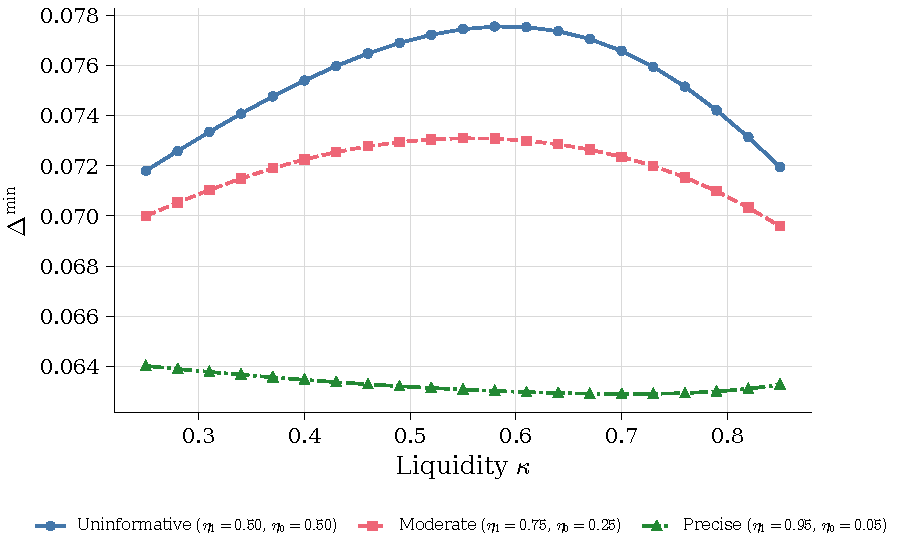
\includegraphics[width=\linewidth]{fig_noisy_rumor.pdf}

\column{0.43\textwidth}
\small
\textbf{Extension (Section 8.3):} Augment market's information with binary rumor $R \in \{0,1\}$:
\begin{itemize}\itemsep0.1em
  \item $\PP(R{=}1 \mid a{=}1) = \eta_1$ (true positive)
  \item $\PP(R{=}1 \mid a{=}0) = \eta_0$ (false positive)
\end{itemize}

Updated posterior:
{\footnotesize
\[
\pi(X,0,R) = \frac{\omega_Q \cdot p_z \cdot \eta_R^Q}{\sum_j \omega_j \cdot p_z \cdot \eta_R^j}
\]}

As $\eta_1 \to 1, \eta_0 \to 0$: converges to FI within $D{=}0$ states.
\end{columns}

\vspace{0.1em}
\footnotesize
Systematic \textbf{flattening} as rumor precision increases: additional information about quiet engagement substitutes for disclosure, further attenuating the liquidity effect.

\returnlink{main:attenuation}{Slide 11: Disclosure Attenuation}
\end{frame}

% ── BACKUP 14: GE disclosure effect ─────────────────────────────────────
\begin{frame}{GE effect of stricter disclosure?}
\hypertarget{backup:GE_disclosure}{}
\small
\begin{block}{Proposition 7 (GE Disclosure Trade-off)}
\vspace{-0.3em}
\[
\frac{d\Delta^{\text{act}}}{d\tau} \approx \underbrace{\frac{\partial\Delta^{\text{act}}}{\partial\tau}\bigg|_{\text{fixed}}}_{\text{Transparency (+)}} + \underbrace{\frac{\partial\Delta^{\text{act}}}{\partial k_D}\cdot\frac{dk_D}{d\tau}}_{\text{Deterrence (---)}}
\]
\vspace{-0.5em}
\end{block}

\begin{columns}[T,onlytextwidth]
\column{0.48\textwidth}
{\small\textbf{Transparency dominates:}}
\begin{itemize}\itemsep0pt
  \item Low $C_0$, moderate $\kappa$
  \item Strict disclosure improves welfare
\end{itemize}

\column{0.48\textwidth}
{\small\textbf{Deterrence dominates:}}
\begin{itemize}\itemsep0pt
  \item High $C_0$
  \item Destroys Quiet Voice, \emph{harms} minorities
\end{itemize}
\end{columns}

\vspace{0.2em}
{\small\textbf{Policy:} SEC 13D filing window reforms must account for deterrence, not just transparency.}

\returnlink{main:policy}{Slide 12: Policy Implications}
\end{frame}

% ── BACKUP 12b: PE vs GE disclosure distinction ────────────────────────
\begin{frame}{PE vs.\ GE: Two disclosure effects}
\hypertarget{backup:PE_vs_GE}{}
\small
\begin{columns}[T,onlytextwidth]
\column{0.48\textwidth}
\textbf{Proposition 6 (Partial Equilibrium):}
\begin{itemize}\itemsep0.1em
  \item \textbf{Fix} cutoffs $(k_1, k_0, k_D)$
  \item Vary $\kappa$ through inference only
  \item Disclosed states ($D{=}1$): $\kappa$-invariant
  \item Inferred states ($D{=}0$): weight $1 - \omega_P$
\end{itemize}
$\Rightarrow$ $|\partial\Delta^{\text{act}}/\partial\kappa|$ \textbf{decreases} as $\omega_P$ rises.

\column{0.48\textwidth}
\textbf{Proposition 7 (General Equilibrium):}
\begin{itemize}\itemsep0.1em
  \item \textbf{Allow} $k_D = k_D(\tau)$ to adjust
  \item Total derivative decomposes:
\end{itemize}
\vspace{-0.3em}
\[
\frac{d\Delta^{\text{act}}}{d\tau} \approx \underbrace{(+)}_{\text{transp.}} + \underbrace{(-)}_{\text{deter.}}
\]
\vspace{-0.3em}
\begin{itemize}\itemsep0.1em
  \item Stricter $\tau$ destroys Quiet Voice
  \item Blockholder may exit rather than disclose
\end{itemize}
\end{columns}

\vspace{0.3em}

{\footnotesize\textbf{Key distinction:} PE shows \emph{why} disclosure attenuates (mechanical: $D{=}1$ states are $\kappa$-free). GE shows \emph{whether} stricter disclosure helps. Low $C_0$ + moderate $\kappa$: transparency dominates. High $C_0$: deterrence dominates.}

\returnlink{main:attenuation}{Slide 11: Disclosure Attenuation}
\end{frame}

% ── CATEGORY DIVIDER: Welfare ────────────────────────────────────────────
\begin{frame}{}
\centering
\vspace{2cm}
{\Large\textbf{Backup: Welfare}}
\end{frame}

% ── BACKUP 15: Welfare decomposition ────────────────────────────────────
\begin{frame}{Distributional or total surplus?}
\hypertarget{backup:welfare}{}
\begin{columns}[T,onlytextwidth]
\column{0.55\textwidth}
\centering

\includegraphics[width=0.95\linewidth]{fig_welfare.pdf}

\column{0.43\textwidth}
\footnotesize
\textbf{Welfare:} $W(\kappa) = W_{\min} + W_B + W_{\text{bid}}$

\vspace{0.1em}
Prices/premia are transfers. Surplus $=$ synergies $+$ improvements $-$ costs.

\vspace{0.1em}
\textbf{Tension:} $\kappa^{\dagger}$ maximizes extraction, deterring marginal efficient takeovers.
$\Rightarrow$ $\kappa^* \neq \kappa^{\dagger}$.
\end{columns}

\returnlink{main:policy}{Slide 12: Policy Implications}
\end{frame}

% ── BACKUP 16: Why minority gains as welfare metric ──────────────────────
\begin{frame}{Why use expected minority takeover gains as the welfare metric?}
\hypertarget{backup:welfare_metric}{}
\footnotesize
\textbf{Grossman \& Hart (1980):} Dispersed minorities benefit only through the takeover \emph{premium}.

\vspace{0.1em}

\textbf{$\Delta^{\min}$ captures:}
\vspace{-0.2em}
\begin{enumerate}\itemsep-0.05em
  \item \emph{Probability} a bid arrives (prices embed inference)
  \item \emph{Premium} conditional on bid (inferred vs.\ observed)
  \item Interaction of these channels through $\kappa$
\end{enumerate}

\vspace{-0.15em}

\textbf{Empirical:} activist returns $\approx$ takeover premia \citep{BravJiangPartnoyThomas2008}. $\Delta^{\min}$ $=$ \emph{ex ante} expected CAR.

\returnlink{main:result}{Slide 10: Main Result}
\end{frame}

% ── CATEGORY DIVIDER: Calibration & Numerical Details ────────────────────
\begin{frame}{}
\centering
\vspace{2cm}
{\Large\textbf{Backup: Calibration \& Numerical Details}}
\end{frame}

% ── BACKUP 17: Baseline parameter values ────────────────────────────────
\begin{frame}{What are your baseline parameter values and why?}
\hypertarget{backup:calibration}{}
\scriptsize
\begin{columns}[T,onlytextwidth]
\column{0.48\textwidth}
\begin{tabular}{@{}lrl@{}}
\toprule
\textbf{Parameter} & \textbf{Value} & \textbf{Rationale} \\
\midrule
$\mu$ (prior mean) & 1.00 & Normalization \\
$\sigma_v$ (value std) & 0.50 & Moderate uncertainty \\
$\sigma_\varepsilon$ (noise std) & 0.50 & $\beta = 0.5$ (equal weight) \\
$\delta$ (discount) & 0.95 & Near-term horizon \\
$\kappa$ (liquidity) & 0.50 & Interior baseline \\
$C_0$ (base cost) & 0.12 & Moderate engagement \\
$\chi$ (cost sensitivity) & 0.50 & Gradual decay \\
\bottomrule
\end{tabular}

\column{0.48\textwidth}
\begin{tabular}{@{}lrl@{}}
\toprule
\textbf{Parameter} & \textbf{Value} & \textbf{Rationale} \\
\midrule
$\rho$ (success prob) & 0.90 & Selective activists \\
$\Delta$ (value-add) & 0.25 & 25\% of $\mu$ \\
$m_0$ (base premium) & 0.10 & 10\% of $\mu$ \\
$m_1$ (success premium) & 0.30 & 30\% of $\mu$ \\
$\bar{S}$ (synergy) & 1.44 & Interior bid prob \\
$K$ (entry cost) & 0.15 & Moderate friction \\
$\sigma_\xi$ (shock vol) & 0.40 & Bidder heterogeneity \\
\bottomrule
\end{tabular}
\end{columns}

\vspace{0.3em}

\textbf{Derived:} $\sigma_s = 0.707$, $\beta = 0.5$, $\tilde{m} = 0.28$, $\tilde{\Delta} = 0.225$.

\vspace{0.2em}

\textbf{Regularity check:} $\delta/\sigma_\xi = 0.95/0.40 = 2.375 < 1/\varphi(0) \approx 2.507$. $\checkmark$ (Assumption A5 satisfied.)

\returnlink{main:engagement}{Slide 6: Engagement \& Bidder Entry}
\end{frame}

% ── BACKUP 18: Full equilibrium outcomes at baseline ─────────────────────
\begin{frame}{Show me the full equilibrium outcomes at baseline.}
\hypertarget{backup:baseline_outcomes}{}
\footnotesize
\textbf{Cutoffs:} $k_1 = k_0 \approx 0.82$, $k_D \approx 2.26$.

\vspace{0.1em}

\begin{center}
\begin{tabular}{ccrrrr}
\toprule
$D$ & $X$ & $P(X,D)$ & $\pi(X,D)$ & $p(X,D)$ & $\bar{m}(X,D)$ \\
\midrule
0 & $-2$ & 0.65 & 0.00 & 0.58 & 0.10 \\
0 & $-1$ & 0.72 & 0.09 & 0.55 & 0.12 \\
0 & $0$  & 0.89 & 0.52 & 0.48 & 0.19 \\
0 & $1$  & 1.04 & 0.78 & 0.43 & 0.24 \\
\midrule
1 & $0$  & 1.14 & 1.00 & 0.39 & 0.28 \\
1 & $1$  & 1.14 & 1.00 & 0.39 & 0.28 \\
1 & $2$  & 1.14 & 1.00 & 0.39 & 0.28 \\
\bottomrule
\end{tabular}
\end{center}

\vspace{0.1em}

\textbf{Key:} (i) $D{=}1$: $\pi = 1$, flat prices; (ii) $D{=}0$: inference gradient; (iii) $D{=}1$ has \emph{lower} bid probability ($\tilde{m} > m_0$).

\returnlink{main:prop3}{Slide 9: Price Decomposition}
\end{frame}

% ── BACKUP 19: Within-regime liquidity effects on posteriors ─────────────
\begin{frame}{What are the within-regime liquidity effects on posteriors?}
\hypertarget{backup:liquidity_posteriors}{}
\small
\textbf{Partial derivatives (Appendix B.7):}

\vspace{0.2em}

\begin{enumerate}\itemsep0.2em
  \item $\frac{\partial\pi(1,0)}{\partial\kappa} = 0$\;---\;
  {\footnotesize $X{=}1, D{=}0$ pins $q{=}0$; mix of Hold/Quiet depends on cutoffs, not $\kappa$.}

  \item $\frac{\partial\pi(0,0)}{\partial\kappa} \le 0$\;---\;
  {\footnotesize Rising $\kappa$ dilutes inference of Quiet Voice; compresses $\pi(0,0)$ toward prior.}

  \item $\frac{\partial\pi(-1,0)}{\partial\kappa} \ge 0$\;---\;
  {\footnotesize Rising $\kappa$ makes $X{=}{-}1$ more likely from Hold/Quiet with bad noise, raising $\pi$.}
\end{enumerate}

\vspace{0.2em}

{\small\textbf{Net effect on $\Delta^{\text{act}}$:} probability-weighted sum across states yields the hump.}

\returnlink{main:prop2}{Slide 8: Proposition 2}
\end{frame}

% ── BACKUP 20: Standing assumptions ──────────────────────────────────────
\begin{frame}{What are the standing assumptions?}
\hypertarget{backup:assumptions}{}
\footnotesize
\begin{center}
\begin{tabular}{clp{6.5cm}}
\toprule
& \textbf{Assumption} & \textbf{Where Used} \\
\midrule
A1 & Normal fundamentals: $v \sim N(\mu, \sigma_v^2)$ & Posterior mean, conditional expectations \\
A2 & Normal signal noise: $s = v + \varepsilon$, $\varepsilon \sim N(0, \sigma_\varepsilon^2)$ & Bayesian updating, cutoff regions \\
A3 & Discrete noise trading: $z \in \{-1,0,+1\}$ & Order flow inference, posterior formulas \\
A4 & Exponential engagement cost: $C(s) = C_0 e^{-\chi z}$ & Single-crossing (Prop.\ 1) \\
A5 & Bounded feedback: $\delta\varphi(0)/\sigma_\xi < 1$ & Price fixed-point uniqueness \\
A6 & Cutoff mapping is a contraction & Equilibrium uniqueness (Prop.\ 4) \\
A7 & Bidder observes $(P, D)$ but not $(X, s, v, a)$ & Information structure, entry rule \\
\bottomrule
\end{tabular}
\end{center}

\vspace{0.3em}

\textbf{Note:} A5 is verifiable ex ante from primitives. A6 is verified numerically (following \citealp{EdmansGoldsteinJiang2015}). All other assumptions are standard.

\returnlink{main:timeline}{Slide 5: Model Timeline}
\end{frame}

\end{document}
